\section{STT-RAM Cache Modeling} \label{sec:model}


\subsubsection{Area Modeling}

MOS-accessed cell corresponds to the typical 1T1R (1-transitor-1-resistor) structure used by many STT-RAM prototypes, in which an NMOS access device is connected in series with the MTJ as shown in Fig.~\ref{fig:1t1r}.  Such an NMOS device turns on/off the access path to the storage element by tuning the voltage applied to its gate.  The MOS-accessed cell usually has the best isolation among neighboring cells due to the property of MOSFET.

\begin{figure}[t]
  \centering
  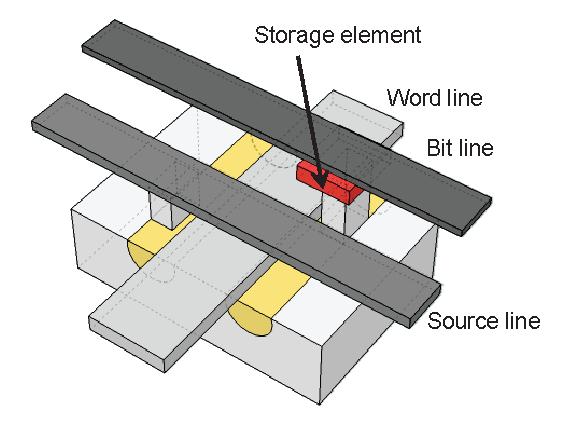
\includegraphics[width=2.0in]{fig/1t1r.eps}
  \caption{Conceptual view of a MOS-accessed cell (1T1J) and its connected word line, bit line, and source line.}
  \label{fig:1t1r}
\end{figure}

In MOS-accessed cells, the size of NMOS is bounded by the current needed by the write operation.  the size of NMOS in each MOS-accessed cell needs to be sufficiently large so that the NMOS has the capability of driving enough write current. The driving current of NMOS, $I_{DS}$ can be first-order estimated as follows,
\begin{equation}
I_{DS}=K\frac{W}{L}\left[\left(V_{GS}-V_{TH}\right)V_{DS}-\frac{V_{DS}^2}{2}\right]  \label{equ:linear}
\end{equation}
if NMOS is working at the linear region; or calculated by
\begin{equation}
I_{DS}=\frac{K}{2}\frac{W}{L}\left(V_{GS}-V_{TH}\right)^2\left(1+\lambda  \label{equ:sat}
V_{DS}\right)
\end{equation}
if NMOS is working at the saturation region.  Hence, no matter in which region NMOS is working, the current driving ability of NMOS is proportional to its width-to-length~(W/L) ratio, which determines the NMOS size.  To achieve high cell density, we model the MOS-accessed cell area by referring to DRAM design rules~\cite{DRAM:6F2}.  As a result, the cell size of a MOS-accessed cell in NVSim is calculated as follows,
\begin{equation}
\mathrm{Area}_{\mathrm{cell,MOS-accessed}}={3\left(W/L+1\right)}(F^2)
\end{equation}
in which the width-to-length ratio (W/L) is determined by Equation~\ref{equ:linear} or Equation~\ref{equ:sat} and the required write current is configured as one of the input values of NVSim. 